\documentclass[14pt, a4paper, oneside]{extarticle}
\usepackage[T2A]{fontenc}
\usepackage[utf8]{inputenc}
\usepackage[russian]{babel}
\usepackage{hyperref}
\usepackage{xcolor}
\usepackage{geometry}
\geometry{top=1cm, bottom=0.5cm, left=1cm, right=1cm}
\usepackage{graphicx}
\usepackage{float}
\usepackage{wrapfig}
\usepackage{fontawesome5}
\usepackage{ragged2e}
\usepackage{microtype}

\hypersetup{
    colorlinks=true,
    allcolors=blue,
    pdfborderstyle={/S/U/W 0},
    allbordercolors=blue
}

\begin{document}

% Фото

%\begin{wrapfigure}{l}{0.18\textwidth}
%	\vspace{\intextsep}
%    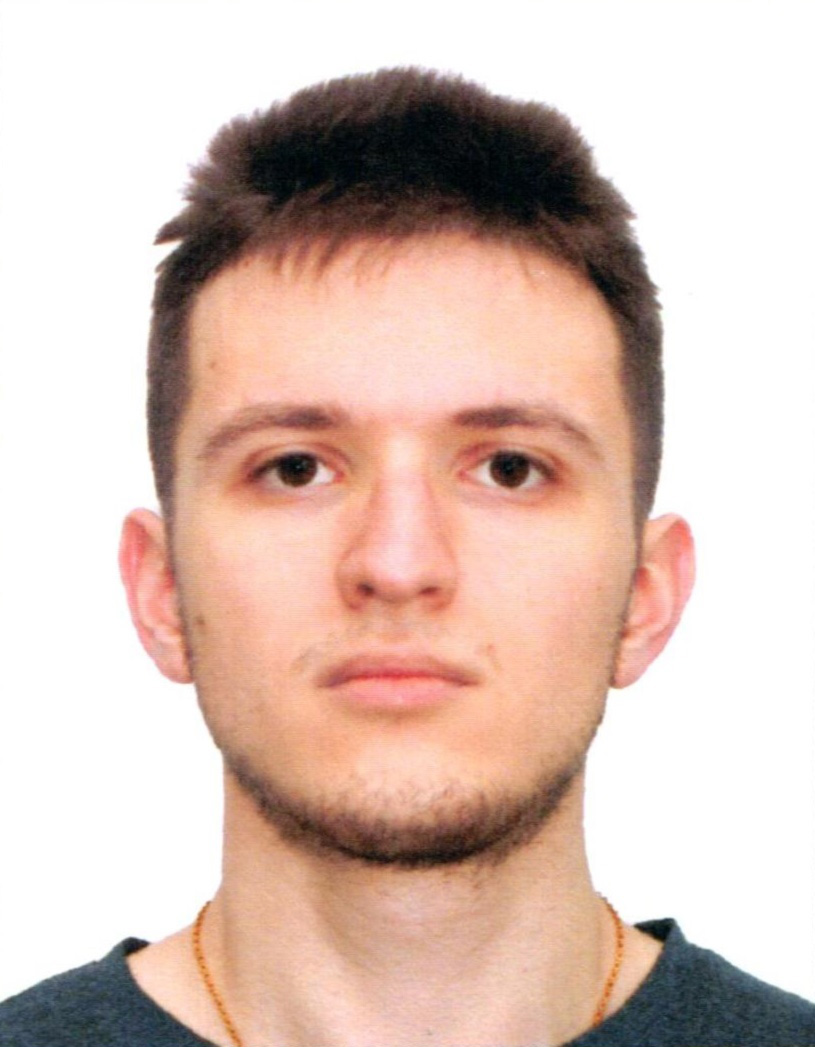
\includegraphics[width=0.18\textwidth]{personal_photo.jpg}
%\end{wrapfigure}

% Заголовок

\begin{center}
    \textbf{\LARGE Куценко Максим Дмитриевич}
    
    \textit{\Large QA-инженер}
\end{center}

\begin{center}
	\vspace{-0.5\intextsep}
	\small
    \faPhone* \space +7 (985) 647-53-50 | \faEnvelope \space maximkuts23@gmail.com | \faGithub \space github.com/Crazy5202 | \faTelegram \space @Crazy523
\end{center}

% Подзаголовок Практический опыт

\begin{flushleft}
	\vspace{-\intextsep}
	\large Практический опыт
\end{flushleft}

\vspace{-0.8\intextsep}
\hrule

%% eComm

\begin{flushleft}
	\vspace{-0.8\intextsep}
	\quad
	\href{https://github.com/Crazy5202/eComm}{\textbf{Бэкенд интернет-магазина (учебный проект)}}
	\hfill
	Москва
\end{flushleft}

\begin{flushleft}
	\vspace{-1\intextsep}
	\quad
	\textit{Московский авиационный институт}
	\hfill
	\textit{\small Фев. 2025 - Июнь 2025}
\end{flushleft}

%%% Список eComm

\vspace{-0.8\intextsep}

\href{https://github.com/Crazy5202/job_application_form/tree/main/portfolio/eComm_C4.pdf}{Микросервисная архитектура решения (C4)}

\begin{itemize}
	\vspace{-0.8\intextsep}
	\item Создание FastAPI сервиса авторизации (SSO) на основе JWT token в cookie
	\vspace{-0.8\intextsep}
	\item Написание логики взаимодействия с СУБД через SQLAlchemy ORM, миграций схемы с Alembic
	\vspace{-0.8\intextsep}
	\item Написание асинхронных unit-тестов для сервисов через pytest
    \vspace{-0.8\intextsep}
    \item Настройка развёртывания проекта на удалённом сервере с Docker
	\vspace{-0.8\intextsep}
	\item Интеграционное и нагрузочное тестирование через Postman
	\vspace{-0.8\intextsep}
    \item Координация команды (4 человека) и ведение бэклога по вопросам тестирования, поддержка проектной документации
\end{itemize}

%% Кинотеатр

\begin{flushleft}
	\vspace{-\intextsep}
	\quad
	\href{https://github.com/Crazy5202/Python_project}{\textbf{Онлайн-кинотеатр (учебный проект)}}
	\hfill
	Москва
\end{flushleft}

\begin{flushleft}
	\vspace{-1\intextsep}
	\quad
	\textit{Московский авиационный институт}
	\hfill
	\textit{\small Сент. 2024 - Дек. 2024}
\end{flushleft}

%%% Список Кинотеатр

\begin{itemize}
    \vspace{-2\intextsep}
    \item Настройка развёртывания проекта на удалённом сервере с Docker
	\vspace{-0.8\intextsep}
	\item Интеграционное и нагрузочное тестирование через Postman
	\vspace{-0.8\intextsep}
	\item UI/UX тестирование
	\vspace{-0.8\intextsep}
    \item Координация команды (4 человека) и ведение бэклога по вопросам тестирования, поддержка проектной документации
\end{itemize}

%% ЭДО

\begin{flushleft}
	\vspace{-0.8\intextsep}
	\quad
	\href{https://github.com/Crazy5202/CM_2024}{\textbf{\smallСервис распознавания подписей и печатей в документах (учебный проект)}}
	\hfill
	Москва
\end{flushleft}

\begin{flushleft}
	\vspace{-1\intextsep}
	\quad
	\textit{Московский авиационный институт, МТС}
	\hfill
	\textit{\small Фев. 2024 - Июнь 2024}
\end{flushleft}

%%% Список ЭДО

\begin{itemize}
    \vspace{-2\intextsep}
    \item Настройка развёртывания проекта на удалённом сервере с Docker
	\vspace{-0.8\intextsep}
	\item Интеграционное и нагрузочное тестирование через Postman
	\vspace{-0.8\intextsep}
	\item UI/UX тестирование
	\vspace{-0.8\intextsep}
    \item Координация команды (9 человек) и ведение бэклога по вопросам тестирования, поддержка проектной
    документации
\end{itemize}

% Подзаголовок Образование

\begin{flushleft}
	\vspace{-\intextsep}
	\large Образование
\end{flushleft}

\vspace{-0.8\intextsep}
\hrule

%% Магистратура

\begin{flushleft}
	\vspace{-0.8\intextsep}
	\quad
	\textbf{Московский авиационный институт}
	\hfill
	Москва
\end{flushleft}

\begin{flushleft}
	\vspace{-\intextsep}
	\quad
	\textit{\footnotesize Магистр, фундаментальная информатика и информационные технологии} 
	%искусственный интеллект и суперкомпьютерное моделирование}
	\hfill
	\textit{\small Авг. 2026 - н.в.}
\end{flushleft}

%% Бакалавриат

\begin{flushleft}
	\vspace{-0.8\intextsep}
	\quad
	\textbf{Московский авиационный институт}
	\hfill
	Москва
\end{flushleft}

\begin{flushleft}
	\vspace{-\intextsep}
	\quad
	\textit{Бакалавр, прикладная математика и информатика}
	\hfill
	\textit{\small Авг. 2022 - Авг. 2026}
\end{flushleft}

% Новая страница

\pagebreak

% Подзаголовок Навыки

\begin{flushleft}
	\vspace{-\intextsep}
	\large Навыки
\end{flushleft}

\vspace{-0.8\intextsep}
\hrule

%% Навыки

\vspace{0.5\intextsep}

\textbf{Языки программирования:} SQL, Python (Flask, FastAPI, SQLAlchemy, Alembic, asyncio, pytest, Selenium), C\slash C++, C\#

\textbf{Языки скриптов:} Bash, Batch/CMD

\textbf{Инфраструктура и интеграции:} Linux, Git, Docker, Jenkins, Postman, Traefik, Debezium, OSI (L2/L3)

\textbf{БД и хранилища:} PostgreSQL, MongoDB, Redis, Elasticsearch, ClickHouse, S3

\textbf{ИИ-инструменты:} n8n, ZCode 

\textbf{Проектирование API, протоколы:} HTTP/HTTPS, REST, Swagger, JSON, XML

\textbf{Наблюдаемость:} Grafana, Prometheus, Loki, Promtail, Logstash, Kibana

\textbf{Очереди сообщений:} Kafka, RabbitMQ

\textbf{Моделирование архитектуры и процессов:} C4, UML, BPMN, ERD

\textbf{Трекинг задач и документация:} Jira, Trello, Confluence, Figma, MS Office

\textbf{Методологии и фреймворки:} Scrum, Kanban, CI/CD

\textbf{Иностранные языки:} Английский C1

% Подзаголовок О себе

\begin{flushleft}
	\vspace{-\intextsep}
	\large О себе
\end{flushleft}

\vspace{-0.8\intextsep}
\hrule

%% О себе
\begin{sloppypar}
	\vspace{0.5\intextsep}
	\quad
	Начинающий QA-инженер с практическим опытом тестирования микросервисных проектов: интеграционное и нагрузочное тестирование API через Postman, UI/UX-проверки, написание асинхронных unit-тестов на pytest, подготовка тестовых окружений и развёртывание проектов на удалённом сервере с Docker. Работал в командах от 4 до 9 человек: вёл бэклог по вопросам тестирования и поддерживал проектную документацию, участвовал в уточнении требований и подготовке тестовых сценариев. 
\end{sloppypar}

\end{document}